\section{Imperfect plate and spheres}
\label{sec:3:imperfect-plates}

In reality, the plate and/or the spheres are not perfectly flat and the surfaces are strewn with imperfections.
This leads to small and local changes in the sphere-plate separation and thus to a marginally altered Casimir energy.
Due to symmetry it is enough to only consider a imperfect plate and a perfectly smooth sphere as the Casimir interactions in the proximity force approximation (PFA) solely depend on the separation $\mathscr{L}$.
To quantify and estimate the changes in the Casimir force due to these surface irregularities, a selection of different and relevant forms of imperfections with amplitude $\Delta \mathscr{L}$ shown in \cref{fig:3:imperfect-plates} have been studied with numerical methods.
\begin{figure}[!htbp]
  \centering
  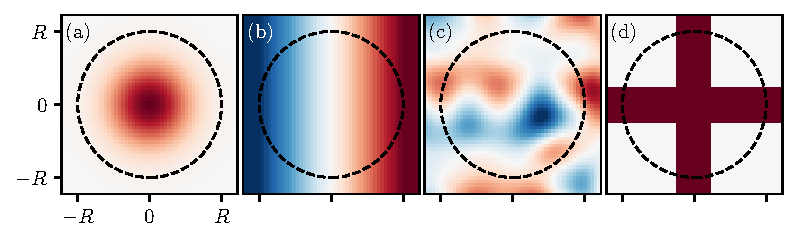
\includegraphics[width=\textwidth]{../figures/casimir/imperfect-plates-advanced.pdf}
  \caption{A selection of imperfect plates. \textbf{(a)} A simple gaussian deformation in the same size as the sphere. \textbf{(b)} Linearly inclining plate or a tilted flat plate. \textbf{(c)} Uneven and noisy but uniformly random surface realized using \textit{Perlin noise} \cite{Perlin_1985}. \textbf{(d)} A cross-shape in the center of the plate.}
  \label{fig:3:imperfect-plates}
\end{figure}
\begin{enumerate}
  \item[\textbf{(a)}] A \textit{gaussian deformation} of the plate can be used to describe a range of possible local imperfections in the size of the sphere. 
  For a small shield ($r_s \approx R$), thermal vibrations look very similar to these deformations, as discussed in \cref{cha:the-shield}.
  A displacement with positive and negative amplitude $\pm \Delta \mathscr{L}$ in the form of a gaussian bell curve is used.

  \item[\textbf{(b)}] For the description of large and thus linearizable imperfections (e.g. like thermal excitations on a large shield $r_s \ll R$), a \textit{linear deflection} is used. This deflection can be also understood as a tilted plate in front of the sphere where one side is much closer to the sphere than the other. For small tilting angles these variations in the Casimir potential cancel out in first order and one expects no significant change in the total attraction force.
  
  \item[\textbf{(c)}] Similarly neglectable should therefore be random noisy but uniformly distributed deformations which are here qualitatively given by the \textit{Perlin noise} function \cite{Perlin_1985}. This type of noise is commonly used in computer science and produces a uniform smooth pseudo-random noise that is often utilized to imitate surface roughness \cite{Perlin_1985}. Equidistant grid-points are defined, each of which is assigned with a pseudo-random gradient. The noise function follows this gradient in the vicinity of a grid-point and the interpolation between points generates smooth transitions. Due to the uniformness, no large deviations from an ideal flat plate is expected.
  
  \item[\textbf{(d)}] A structure on the shield, like e.g. a \textit{centered cross} might improve stability and rigidity of the shield. Thermal vibrations could be reduced by such a design but the effect and amplification of the Casimir interaction has to be investigated.
\end{enumerate}
The resulting Casimir potentials between a macroscopic sphere and the imperfect surfaces were numerically calculated in the PFA and are shown in \cref{fig:3:casimir-imperfect-plates}.
\begin{figure}[!htbp]
  \centering
  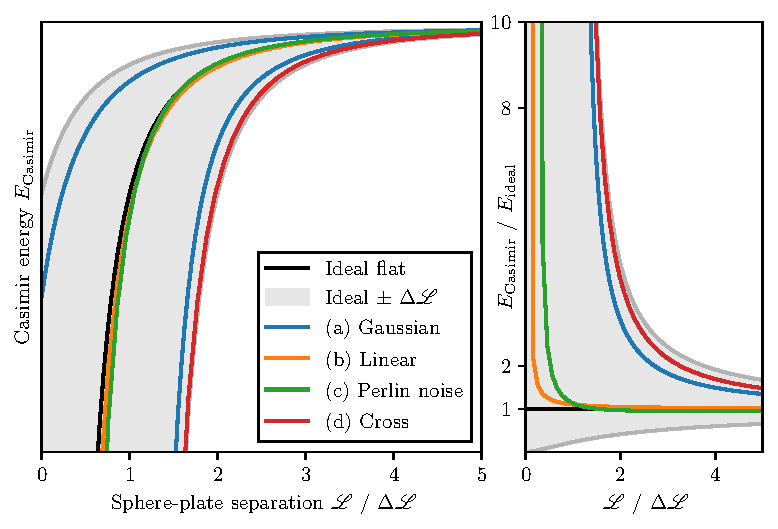
\includegraphics[width=\textwidth]{../figures/casimir/casimir-potential-imperfect-plates-relative.pdf}
  \caption{Casimir energy for the different imperfect plates shown in \cref{fig:3:imperfect-plates}. The dashed-blue line represents a negative gaussian displacement reducing the overall Casimir attraction. The shaded region is given by an ideal plate separated by a distance of $\mathscr{L}_0 \pm \Delta\mathscr{L}$ from the sphere where $\mathscr{L}_0$ is the original separation. It becomes evident that in the limit of $\mathscr{L}\rightarrow\infty$, all local imperfections are neglectable.}
  \label{fig:3:casimir-imperfect-plates}
\end{figure}
As logically expected, all variations are upper bounded by moving the ideal flat plate closer (or farther) to the sphere by a distance $\Delta \mathscr{L}$.
For the gaussian distribution, the overestimation is not particularly large.
An evenly tilted plate as well as a uniformly noisy plate do not change the Casimir interactions noticeably even at small separations.
If the plate and sphere are far apart ($\mathscr{L} \gg R$), all local imperfections are neglectable, as their relative effect decreases and becomes less noticeable.
However, the considerations made in this section are particularly important for small shields the size of the particles and close distances.